\section{Smooth Optimization} 

	The first thing you learn about gradients in multivariate calculus is that \hyperref[mul-thm:gradient_increase]{they point in the step of steepest ascent}. Generally, you can think of the function you're trying to minimize as a ``landscape.'' This inspires a greedy approach to simply walk in this direction $\nabla f(x)$ to maximize a function (or walk in the opposite direction $-\nabla f(x)$). This gives the following. 

  \begin{definition}[Gradient Descent]
    \label{def:gradient-descent}
		Given a differentiable $f: \mathbb{R}^d \to \mathbb{R}$, and $x_0 \in \mathbb{R}^d$, \textbf{gradient descent} defines the sequence 
		\begin{equation}
			x_{k} = x_{k - 1} - \eta \nabla f(x_{k-1})
		\end{equation}
		where $\eta$ is known as the \textbf{learning rate}. 

    \begin{algorithm}[H]
			\begin{algorithmic}[1]  % The [1] adds line numbers
				% Input/Output documentation
				\Require{Function $f(x)$, initialization $x_0$, learning rate}
				\Procedure{GradientDescent}{$f, x_0$}
					\State $x \gets x_0$ 
					\While{not converged} 
						\State $x \gets x - \eta \nabla f(x)$
					\EndWhile
					\State \Return $x$ 
				\EndProcedure
			\end{algorithmic}
    \end{algorithm} 
  \end{definition}

  The algorithm may not converge if $\alpha$ (the step size) is too high, since it may overshoot. This can be solved by reducing the $\alpha$ with each step, using \textit{schedulers}. 

  Ideally, we would want to have a variable step size $h(t)$ so that $h \rightarrow 0$ as $t \rightarrow + \infty$. 

  \begin{algo}[Decay on Plateau Learning Rate]
    Basically, this says that if the loss doesn't decrease for the past $p$ epochs, then decrease the learning rate $\eta \gets \gamma \cdot \eta$. 
    \begin{algorithm}[H]
    \label{alg:lr_decay_plateau}
    \begin{algorithmic}[1]  % The [1] adds line numbers
      \Require{Patience $p$, decay rate $0 < \gamma < 1$, initial $\theta_0$, loss $L$}

      \Procedure{LRDecayOnPlateau}{$p, \gamma, \theta, \eta$}
        \State $\text{best\_loss} \gets L(\theta)$ 
        \State $\text{bad\_epochs} \gets 0$
        \While{not converged} 
          \State $\theta \gets \theta - \eta \nabla L(\theta)$ 
          \If{$L(\theta) < \text{best\_loss}$}  
            \State $\text{best\_loss} \gets L(\theta)$ 
            \State $\text{bad\_epochs} \gets 0$
          \Else 
            \State $\text{bad\_epochs} \gets \text{bad\_epochs} + 1$
          \EndIf 
          \If{$\text{bad\_epochs} \geq p$} 
            \State $\eta \gets \eta \cdot \gamma$ 
            \State $\text{bad\_epochs} \gets 0$
          \EndIf 
        \EndWhile
        \State \Return $\theta, \eta$
      \EndProcedure
    \end{algorithmic}
    \end{algorithm}
  \end{algo}


	This is a pretty simple approach, but this raises so many questions. For example, can we ensure convergence? Will it actually land in the minimum? 

	\begin{definition}[$\epsilon$-Critical Point]
		For differentiable function $f: \mathbb{R}^d \to \mathbb{R}$, $x \in \mathbb{R}^d$ is an \textbf{$\epsilon$-critical point} if 
		\begin{equation}
		  \|\nabla f(x)\| \leq \epsilon
		\end{equation}
	\end{definition}

	A function being \hyperref[mul-def:ck_functions]{$C^k$} is great, but often we wish to bound the derivatives as well. 

	\begin{definition}[$L$-Smooth]
	  A function $f: \mathbb{R}^d \to \mathbb{R}$ is \textbf{$L$-smooth} if the gradient is $L$-Lipschtiz. 
		\begin{equation}
		  \| \nabla f(x) - \nabla f(y) \| \leq L \|x - y\|
		\end{equation}
	\end{definition}

	\begin{theorem}[Taylor's 1st Order Bound]
		If $f: \mathbb{R}^d \to \mathbb{R}$ is $C^1$ and $L$-smooth, then 
		\begin{equation}
			|f(y) - f(x) - \langle \nabla f(x), y - x \rangle | \leq \frac{L}{2} \|y - x\|^2
		\end{equation}
	\end{theorem}
	\begin{proof}
		Let $y = x + s$ and define $\theta: [0, 1] \to \mathbb{R}, \theta(t) = f(w + ts)$. Since $f \in C^1$, $f^\prime$ is continuous and hence Riemann integrable. By the \hyperref[real-thm:ftc2]{2nd fundamental theorem of calculus}, we can write 
		\begin{align}
			|f(x + s) - f(x) - \nabla f(x)^T s| & = \bigg| \theta(0) + \int_0^1 \theta^\prime (t) \,dt - \theta(0) - \nabla f(x)^T s \bigg|  \\ 
																					& = \bigg| \int_0^1 \langle \nabla f(x + ts) - \nabla f(x), s \rangle \,dt \\ 
																					& \leq \int_0^1 | \langle \nabla f(x + ts) - \nabla f(x), s \rangle | \,dt \\ 
																					& \leq \int_0^1 \| \nabla f(x + ts) - \nabla f(x) \| \|s\| \,dt \\ 
																					& \leq \int_0^1 L \|ts\| \|s\|\,dt \\ 
																					& = \frac{1}{2} L \|s\|^2
		\end{align}
	\end{proof}

	\begin{corollary}[Taylor's 2nd Order Bound]
		If $f: \mathbb{R}^d \to \mathbb{R}$ is $C^2$ and has a $Q$-Lipschitz Hessian $\nabla^2 f$, then 
	\end{corollary}
	\begin{proof}
		We can use FOTC twice since $f$ is $C^2$. So, 
		\begin{align}
			\theta(1) & = \theta(0) + \int_0^1 \theta^\prime (t) \,dt \\ 
								& = \theta(0) + \int_0^1 \bigg( \theta^\prime(0) + \int_0^t \theta^{\prime\prime}(\alpha) \,d\alpha \bigg) \, dt \\ 
								& = \theta(0) + \theta^\prime (0) + \int_0^1 \int_0^t \theta^{\prime\prime} (\alpha) \,d\alpha \,dt 
		\end{align}
		Note that 
		\begin{equation}
			\int_0^1 \int_0^t \theta^{\prime\prime} (0) \,d\alpha \,dt = \theta^{\prime\prime} (0) \int_0^1 \int_0^t \,d\alpha \,dt = \frac{1}{2} \theta^{\prime\prime} (0)
		\end{equation}
		Therefore, 
		\begin{align}
			\bigg| f(x + s) & - f(x) - \nabla f(x)^T s - \frac{1}{2} s^T \nabla^2 f(x) s \bigg| \\ 
											& = \bigg| \theta(0) + \theta^{\prime} (0) + \int_0^1 \int_0^t \theta^{\prime\prime}(\alpha) \,d\alpha \,dt - \theta(0) - \theta^\prime (0) - \frac{1}{2} \theta^{\prime\prime} (0) \bigg| \\ 
											& = \bigg| \int_0^1 \int_0^t \theta^{\prime\prime} (\alpha) \,d\alpha \,dt - \int_0^1 \int_0^t \frac{1}{2} \theta^{\prime\prime}(0) \,d\alpha \,dt \bigg| \\ 
											& = \bigg| \int_0^1 \int_0^t s^T \big( \nabla^2 f(x + \alpha s) - \nabla^2 f(x) \big) s \,d\alpha \,dt \bigg| \\ 
											& \leq \int_0^1 \int_0^t \big| s^T \big( \nabla^2 f(x + \alpha s) - \nabla^2 f(x) \big) s \big| \,d\alpha \,dt \\
											& \leq \int_0^1 \int_0^t \big\| \nabla^2 f(x + \alpha s) - \nabla^2 f(x) \big\|_{op} \|s\|^2 \,d\alpha \,dt \\
											& \leq \int_0^1 \int_0^t Q \|\alpha s\| \|s\|^2 \,d\alpha \,dt \\
											& = Q \|s\|^3 \int_0^1 \int_0^t \alpha \,d\alpha \,dt \\
											& = \frac{1}{6} Q \|s\|^3
		\end{align}
	\end{proof}

	With this result, we can see that 
	\begin{equation}
		f(x) \leq f(w) + \langle \nabla f(w), x - w \rangle + \frac{L}{2} \|x - w\|^2
	\end{equation}
	This is useful since it upper-bounds a potentially complicated nonlinear function by a simple quadratic function. 

	\begin{definition}[$\mu$-Strongly Convex]
		A function $f: \mathbb{R}^d \to \mathbb{R}$ is \textbf{$\mu$-strongly convex} if for all $w, y \in \mathbb{R}^d$, 
		\begin{equation}
			f(y) \geq f(w) + \langle \nabla f(w), y - w \rangle + \frac{\mu}{2} \|y - w\|^2
		\end{equation}
		Note that $f$ is convex when $\mu = 0$. 
	\end{definition}

	An algorithmic design principle that we will follow is that instead of minimizing $f$ directly, we iteratively minimize an approximation of $f$ centered at the previous iterate. We will use this principle over and over again. Therefore, let's start with this iterative procedure. 
	\begin{equation}
		w_{k+1} \gets \argmin_w \Phi_k (w) = \argmin_w \bigg\{ \underbrace{\langle \nabla f(w_k), w - w_k \rangle}_{\text{linear approximation}} + \underbrace{\frac{1}{\eta_k} \|w - w_k\|^2}_{\text{anchor}} \bigg\}
	\end{equation}
	Note that the quadratic term is a regularizer that prevents us from moving too far from the current point $w_k$. This actually turns out to be gradient descent when we look at the first order optimality conditions. Recall that at a local minimum of a differentiable function, the gradient must vanish. So, 
	\begin{equation}
		0 = \nabla \Phi_k (w_{k+1}) = \nabla f(w_k) + \frac{1}{\eta_k}(w_{k+1} - w_k) \implies w_{k+1} = w_k - \eta_k \nabla f(w_k)
	\end{equation}
	So $\eta$ is sort of like the step size. Let's try to show that this is a good idea. 

	\begin{lemma}[Descent Lemma]
		Let $f$ be $L$-smooth and $\eta \in (0, \dfrac{2}{L})$. Then, 
		\begin{equation}
			f(w - \eta \nabla f(w)) \leq f(w) - \eta \big(1 - \frac{L \eta}{2} \big) \|\nabla f(w)\|^2
		\end{equation}
	\end{lemma}
	\begin{proof}
	  This follows from Taylor's with $y = w - \eta f(w)$, since 
		\begin{align}
			f(y) - f(w) + \eta \|\nabla f(w)\|^2 & = f(y) - f(w) + \langle \nabla f(w), y - w \rangle \\ 
																					 & \leq \frac{L}{2} \|y - w\|^2 \\ 
																					 & = \frac{L \eta^2}{2} \| \nabla f(w)\|^2
		\end{align}
	\end{proof}

	\begin{theorem}[Spiral]
		\label{thm:spiral}
		Suppose that $f$ is $L$-smooth and $\inf{f} > -\infty$. Consider the iterates 
		\begin{equation}
			w_{k+1} \gets w_k - \frac{1}{L} \nabla f(w_k)
		\end{equation}
		Then, 
		\begin{equation}
			\min_{k \in [T - 1]} \|\nabla f(w_k) \| \leq \sqrt{ \frac{2L \big( f(w_0) - \inf{f} \big)}{T}}
		\end{equation}
	\end{theorem}
	\begin{proof}
	  
	\end{proof}

	\begin{theorem}[Quadratic Growth]
		Suppose that $f$ is $\mu$-strongly convex. Then, $f$ has a unique minimizer $w^\ast$, and for all $w \in \mathbb{R}^d$, 
		\begin{equation}
			\frac{\mu}{2} \|w - w^\ast\|^2 \leq f(w) - f(w^\ast)
		\end{equation}
	\end{theorem}

	\begin{theorem}[Lightning]
	  Suppose that $f$ is $L$-smooth and $\mu$-strongly convex. Then, the iterates of GD satisfy 
		\begin{equation}
			f(w_k) - f(w^\ast) \leq \bigg( 1 - \frac{\mu}{L} \bigg)^k \big( f(w_0) - f(w^\ast) \big) 
		\end{equation}
	\end{theorem}

	A simply computation yields that if we want to reach 
	\begin{equation}
	  f(w_T) - f(w^\ast) \leq \epsilon
	\end{equation}
	then it suffices to take 
	\begin{equation}
		T \geq \frac{L}{\mu} \ln\bigg( \frac{f(w_0) - f(w^\ast)}{\epsilon} \bigg)
	\end{equation}
	Further quadratic growth ensures 
	\begin{equation}
		\|w_T - w^\ast\| \leq \frac{2 \epsilon}{\mu}
	\end{equation}

	Note that for \hyperref[thm:spiral]{theorem spiral}, we needed $T \geq \frac{2L}{\epsilon^2} \big( f(w_0) - f(w^\ast) \big)$ for $f(w_T) - f(w^\ast) \leq \epsilon$. If $\epsilon = 10^{-6}$, then this means that $e^{-2} = 10^12$ while $\ln(\frac{1}{\epsilon}) \approx 14$. 

	Thus, how fast GD converges is dictated by the ratio 
	\begin{equation}
		\kappa = \frac{L}{\mu} \in [1, \infty]
	\end{equation}
	known as the \textbf{condition number}. Therefore, for general smooth functions, we can merely find critical points at a rather slow rate $O(\epsilon^{-2})$. If we want to guarantee fast convergence towards a minimizer, we need additional geometric structure. For a long time, most of the ``additional geometric structure'' optimizers used to prove guarantees amounted to strong convexity. In the last couple of decades, that has changed. 

	\begin{definition}[Polyak-Lojasiewicz Inequality]
		A differentiable function $f: \mathbb{R}^d \to \mathbb{R}$ satisfies the \textbf{PL-inequality}\footnote{This was published in 1963 and was ignored until 2016.} if there exists a $\mu > 0$ s.t. 
		\begin{equation}
			\mu \big( f(x) - \inf{f} \big) \leq \frac{1}{2} \| \nabla f(x) \|^2 \text{ for all } x \in \mathbb{R}^d
		\end{equation}
	\end{definition}

	This is a relatively strong aassumption, and in particular it yields that 
	\begin{equation}
		\nabla f(x) = 0 \implies f(x) = \inf{f}
	\end{equation}
	Nonetheless, it generalizes the notion of strong convexity. 

	\begin{lemma}[Strong Convexity Implies PL-Inequality]
		Suppose $f: \mathbb{R}^d \to \mathbb{R}$ is differentiable and $\mu$-strongly convex. Then, it satisfies $\mu$-PL. Further, there exists a nonconvex smooth function that satisfies $\mu$-PL. 
	\end{lemma}
	\begin{proof}
	  
	\end{proof}

	\begin{theorem}[Double Lightning]
		Suppose that $f$ is $L$-smooth and satisfies $\mu$-PL. Then, the iterates of GD with $\eta_k = \frac{1}{L}$ satisfy 
		\begin{equation}
			f(w_k) - \inf(f) \leq \bigg( 1 - \frac{\mu}{L} \bigg)^k \big( f(w_0) - f(w^\ast) \big) 
		\end{equation}
	\end{theorem}

	\begin{theorem}
		Suppsoe that $f$ is differentiable, $A \in \mathbb{R}^{m \times d}$ and $b \in \mathbb{R}^m$. Define 
		\begin{equation}
		  \varphi(x) = f(Ax + b)
		\end{equation}
		Then, the following hold. 
		\begin{enumerate}
			\item If $f$ is $L$-smooth, then $\varphi$ is $(L\|A\|^2_{\mathrm{op}})$-smooth. 
			\item If $f$ satisfies $\mu$-PL and $A$ is onto, $\varphi$ satisfies $(\mu \lambda_{\mathrm{min}} (AA^T))$-PL, where $\lambda_{\mathrm{min}}  = \inf_{\|v\| = 1} v^T A A^T v$. 
		\end{enumerate}
	\end{theorem}
	\begin{proof}
	  
	\end{proof}

\subsection{Momentum and Accelerated Gradient Descent}

  \begin{algo}[Stochastic Gradient Descent with Momentum]
    This modifies vanilla SGD by keeping a running velocity term that accumulates past gradients, which smooths updates and helps escape sharp local minima. 
    \begin{algorithm}[H]
    \label{alg:sgd_momentum}
    \begin{algorithmic}[1]  % The [1] adds line numbers
      \Require{Learning rate $\eta$, momentum $0 \leq \mu < 1$, initial parameters $\theta_0$, loss $L$}

      \Procedure{SGDMomentum}{$\eta, \mu, \theta$}
        \State $v \gets 0$ \Comment{Initialize velocity}
        \While{not converged}
          \State $v \gets \mu v + \nabla L(\theta)$        \Comment{Decay prev. velocity and add in gradient (acceleration)}
          \State $\theta \gets \theta - \eta v$
        \EndWhile
        \State \Return $\theta$
      \EndProcedure
    \end{algorithmic}
    \end{algorithm}
  \end{algo}

  \begin{algo}[Stochastic Gradient Descent with Nesterov Momentum]
    Nesterov momentum modifies standard momentum by computing the gradient at the \emph{lookahead} position $\theta - \eta \mu v$, leading to faster convergence in practice. 
    \begin{algorithm}[H]
    \label{alg:sgd_nesterov}
    \begin{algorithmic}[1]  % The [1] adds line numbers
      \Require{Learning rate $\eta$, momentum $0 \leq \mu < 1$, initial parameters $\theta_0$, loss $L$}

      \Procedure{SGDNesterov}{$\eta, \mu, \theta$}
        \State $v \gets 0$ \Comment{Initialize velocity}
        \While{not converged}
          \State $g \gets \nabla L(\theta - \eta \mu v)$ \Comment{Lookahead gradient}
          \State $v \gets \mu v + g$
          \State $\theta \gets \theta - \eta v$
        \EndWhile
        \State \Return $\theta$
      \EndProcedure
    \end{algorithmic}
    \end{algorithm}
  \end{algo}

\subsection{Block Coordinate Descent} 

  \begin{algo}[Block Gradient Descent]
    Block Gradient Descent partitions the parameter vector $\theta$ into $m$ disjoint blocks. At each iteration, it selects one block (cyclically or randomly) and updates only that block's parameters using the gradient, while keeping the other blocks fixed. 
    \begin{algorithm}[H]
    \label{alg:block_gd}
    \begin{algorithmic}[1]  % The [1] adds line numbers
      \Require{Learning rate $\eta$, number of blocks $m$, partition $\theta = (\theta^{(1)}, \dots, \theta^{(m)})$, loss $L$}

      \Procedure{BlockGradientDescent}{$\eta, \{\theta^{(j)}\}_{j=1}^m$}
        \State $t \gets 0$
        \While{not converged}
          \State $j \gets \text{SelectBlock}(t, m)$ \Comment{e.g., cyclic: $j = (t \bmod m) + 1$}
          \State $\theta^{(j)} \gets \theta^{(j)} - \eta \nabla_{\theta^{(j)}} L(\theta^{(1)}, \dots, \theta^{(m)})$
          \State $t \gets t + 1$
        \EndWhile
        \State \Return $\theta$
      \EndProcedure
    \end{algorithmic}
    \end{algorithm}
  \end{algo}

\subsection{Subgradient Methods}

  It is well known that the mean square error of a linear map is convex. However, when we impose the L1 penalty, the loss function is now not differentiable at $\mathbf{0}$. Therefore, we must introduce the notion of a subgradient. 

  \begin{definition}[Subgradient]
    The subgradient of a convex function $f: U \subset \mathbb{R}^n \rightarrow \mathbb{R}$ is any linear map $\mathbf{A} (x): \mathbb{R}^n \rightarrow \mathbb{R}$ such that 
    \begin{equation}
      f(\mathbf{y}) \geq f(\mathbf{x}) + \mathbf{A}(\mathbf{x}) (\mathbf{y} - \mathbf{x})
    \end{equation}
    for any $\mathbf{y} \in U$. The set of all subgradients at $\mathbf{x}$ is called the \textbf{subdifferential} defined 
    \begin{equation}
      \partial f (\mathbf{x}) = \{ \mathbf{A} \in \mathbb{R}^n \mid \mathbf{A} \text{ is a subgradient of } f \text{ at } \mathbf{x} \}
    \end{equation}
  \end{definition}

  The subgradient also acts as a linear approximation of $f$, but now at nondifferentiable points of convex functions, we have a set of linear approximations. It is clear that the subgradient at a differentiable point is uniquely the gradient ($\partial f(\mathbf{x}) = \{ \nabla f(\mathbf{x})$), but for places like the absolute value, we can have infinite linear approximations. 
  \begin{center}
    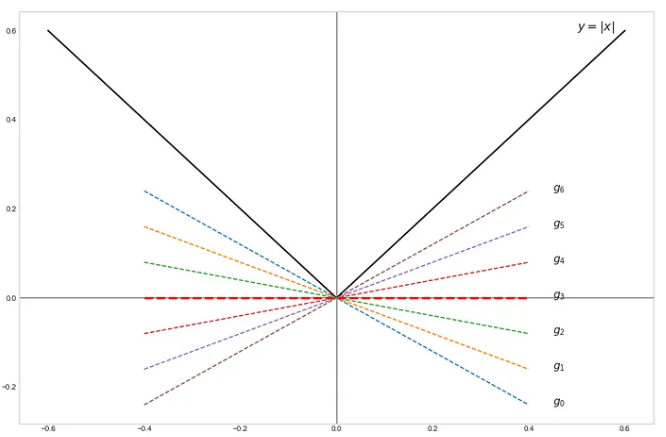
\includegraphics[scale=0.4]{img/subgradient_of_abs.png}
  \end{center}
  Given the subdifferential, thus the optimality condition for any convex $\mathbf{f}$ (differentiable or not) is
  \begin{equation}
    f(\mathbf{x}^\ast) = \min_{\mathbf{x}} f(\mathbf{x}) \iff \mathbf{0} \in \partial f(\mathbf{x}^\ast)
  \end{equation}
  known as the subgradient optimality condition, which clearly implies 
  \begin{equation}
    f(\mathbf{y}) \geq f(\mathbf{x}^\ast) + \mathbf{0}^T (\mathbf{y} - \mathbf{x}^\ast) = f(\mathbf{x}^\ast)
  \end{equation}

  \begin{example}
    The subdifferential of the absolute value function $f(x) = |x|$ at any given $x$ is 
    \begin{equation}
      \partial f(x) = \begin{cases} 1 & \text{ if } x > 0 \\ [-1, 1] & \text{ if } x = 0 \\ -1 & \text{ if } x < 0 \end{cases}
    \end{equation}
  \end{example}

\subsection{Proximal Gradient Methods}

  \begin{definition}[Proximal Operator]
    Given a lower semicontinuous convex function $f$ mapping from Hilbert space $X$ to $[-\infty, +\infty]$, its \textbf{proximal operator} associated with a point $u$ is defined 
    \begin{equation}
      \prox_{f, \tau} (u) = \argmin_{x} \bigg( f(x) + \frac{1}{2\tau} ||x - u||^2 \bigg)
    \end{equation}
    where $\tau > 0$ is a parameter that scales the quadratic term. This is basically the point that minimizes the sum of $f(x)$ and the square of the Euclidean distance between $x$ and $u$, scaled by $1/2\tau$. 
  \end{definition}

  Now given the loss function $L (\boldsymbol{\theta}) = L_{\mathrm{obj}} (\boldsymbol{\theta}) + L_{\mathrm{reg}} (\boldsymbol{\theta})$, we want to compute the proximal operator on the regularization loss and update that with the gradient of the smooth objective loss. 
  \begin{equation}
    \boldsymbol{\theta}^{(k+1)} = \prox_{L_{\mathrm{reg}}, \tau} \big[ \boldsymbol{\theta}^{(k)} - \tau \nabla L_{\mathrm{obj}} (\boldsymbol{\theta}^{(k)}) \big]
  \end{equation}
  Let's compute the proximal operator of the L1 loss $h(\boldsymbol{\theta}) = \lambda ||\boldsymbol{\theta}||_1$. We can parameterize this loss by the $\lambda$, so we will use the notation $\prox_{\lambda, \tau}$ rather than $\prox_{h, \tau}$. 
  \begin{align*}
    \prox_{\lambda, \tau} (\mathbf{u}) & = \argmin_{\boldsymbol{\theta}} \bigg( \lambda ||\boldsymbol{\theta}||_1 + \frac{1}{2\tau} ||\boldsymbol{\theta} - \mathbf{u}||_2^2 \bigg) \\
    & = \argmin_{\boldsymbol{\theta}} \bigg( \sum_{i=1}^n \lambda |\theta_i| + \frac{1}{2\tau} (\theta_i - u_i)^2 \bigg) 
  \end{align*}
  These are separable functions that can be decoupled and optimized component-wise. So, we really just want to find 
  \begin{equation}
    \theta_i^\ast = \argmin_{\theta_i} \bigg( \lambda |\theta_i| + \frac{1}{2\tau} (\theta_i - u_i)^2 \bigg)
  \end{equation}
  The sum of convex functions is convex, and so we should differentiate it and find where the gradient is $0$ to optimize it. 
  \begin{enumerate}
    \item When $\theta_i > 0$, then we minimize $\lambda \theta_i + \frac{1}{2\tau} (\theta_i - u_i)^2$, so taking the gradient and setting to $0$ gives 
    \begin{equation}
      \theta_i = u_i - \lambda \tau
    \end{equation}
    subject to the constraint that $\theta_i > 0$, or equivalently, that $u_i > \lambda \tau$. 

    \item When $\theta_i < 0$, then we minimize $-\lambda \theta_i + \frac{1}{2\tau} ( \theta_i - u_i)^2$, so taking the gradient and setting to $0$ gives 
    \begin{equation}
      \theta_i = u_i + \lambda \tau
    \end{equation}
    subject to the constraint that $\theta_i < 0$, or equivalently, that $u_i < -\lambda \tau$. 

    \item When $\theta_i = 0$, then we minimize $\lambda |\theta_i| + \frac{1}{2\tau} (\theta_i - u_i)^2$, which doesn't have derivative at $\theta_i = 0$. So, we can compute the subdifferential of it to get 
    \[0 \in \partial \bigg( \lambda |\theta_i| + \frac{1}{2\tau} (\theta_i - u_i)^2 \bigg) = \lambda \partial (|\theta_i|) + \frac{1}{\tau} (\theta_i - u_i)\]
    Now at $\theta_i = 0$, the subdifferential can be any value in $[-1, 1]$, and the above reduces to 
    \begin{equation}
      0 \in \lambda [-1, 1] - \frac{1}{\tau} u_i
    \end{equation}
    this is equivalent to saying that $u_i/\tau$ is contained in the interval $[-\lambda, \lambda]$, meaning that $u_i \in [-\lambda \tau, \lambda \tau]$. 
  \end{enumerate}

  Ultimately we get that 
  \begin{equation}
    \prox_{\lambda, \tau} (u) = \begin{cases} u - \lambda \tau & \text{ if } u > \lambda \tau \\ 0 & \text{ if } |u| \leq \lambda \tau \\ u + \lambda \tau & \text{ if } u < - \lambda \tau \end{cases}
  \end{equation}
  which can be simplified to 
  \begin{equation}
    \prox_{\lambda, \tau} (u) = \mathrm{sign}(u) \max\{ |u| - \lambda \tau, 0)
  \end{equation}

\subsection{Stochastic Gradient Descent} 

  Now let's go back to gradient descent. Usually, in machine learning, we are trying to optimize a parameteric model $\mathcal{P} = \{ \mathbb{P}_\theta \mid \theta \in \Theta\}$ over a dataset $\mathcal{D} = \{x_i\}_{i=1}^n$., For example, our estimator in the maximum-likelihood approach will be 
  \begin{equation}
    \delta(\mathcal{D}) = \argmax_{\theta} L(\theta \mid \mathcal{D}) = \log p(\mathcal{D} \mid \theta)
  \end{equation}
  for some loss function $L$. 

  If we assume that the samples are iid, then we can decompose the gradient as 
  \begin{equation}
    \nabla_\theta \log{p(\mathcal{D} \mid \theta)} = \sum_i \nabla_\theta \log{p(d_i \mid \theta)}
  \end{equation}
  which scales linearly with the size of a dataset. This is not scalable with extremely large datasets, and so we must remove this $O(n)$ term. Intuitively, we can think of approximating this gradient by taking a minibatch $b$ of $\mathcal{D}$ and computing the gradient only across that minibatch. 

  \begin{theorem}[Minibatch Gradient is an Unbiased Estimator]
    Let us take a minibatch of $b$ samples $\mathcal{B} \subset \mathcal{D}$ without replacement, where $b << D$. Then, our approximation of the gradient of the log likelihood
    \begin{equation}
       \nabla_\theta \log{p (\mathcal{B} \mid \theta)} \coloneqq \frac{1}{b} \sum_{x \in \mathcal{B}} \nabla_\theta \log{p(x \mid \theta)}
    \end{equation}
    is an unbiased estimator of the true gradient $\nabla_\theta \log{p(\mathcal{D} \mid \theta)}$. That is, setting $\mathcal{M}$ as a random variable of samples over $\mathcal{D}$, we have 
    \begin{equation}
      \mathbb{E}_{\mathcal{M}} [\nabla \mathcal{L}_{\mathcal{M}} (\mathbf{w})] = \nabla \mathcal{L} (\mathbf{w})
    \end{equation}
  \end{theorem}
  \begin{proof}
    We use linearity of expectation for all $\mathcal{M} \subset \mathcal{D}$ of size $M$. 
  \end{proof} 

  This also has the additional advantage of saving memory. You don't have to load in the gradients for the whole dataset (which may be a few TB), and can allocate just enough memory for each batch (perhaps a few GB). 

  \begin{algo}[Stochastic Gradient Descent]

    \begin{algorithm}[H]
    \label{alg:stochacistic-gradient-descent}
    \begin{algorithmic}[1]  % The [1] adds line numbers
      % Input/Output documentation
      \Require{Function $L(\theta)$, initialization $\theta_0$, learning rate, batch size $b$, dataset $\mathcal{D}$}
      \Procedure{StochasticGradientDescent}{$f, \theta_0, b$}
        \State $\theta \gets \theta_0$ 
        \While{not converged} 
          \State Sample minibatch $\mathcal{B} \subset \mathcal{D}$. 
          \State $\theta \gets \theta - \eta \nabla_\theta \log p(\mathcal{B} \mid \theta)$ 
        \EndWhile
        \State \Return $\theta$
      \EndProcedure
    \end{algorithmic}
    \end{algorithm} 
  \end{algo} 

  \begin{example}[Linear Regression]
    We have assumed knowledge of gradient descent in the back propagation step in the previous section, but let's revisit this by looking at linear regression. Given our dataset $\mathcal{D} = \{\mathbf{x}^(n), y^{(n)}\}$, we are fitting a linear model of the form 
    \begin{equation}
      f(\mathbf{x}; \mathbf{w}, b) = \mathbf{w}^T \mathbf{x} + b
    \end{equation} 
    The squared loss function is 
    \begin{equation}
      \mathcal{L}(\mathbf{w}, b) = \frac{1}{2} \sum_{n=1}^N \big( y - f(\mathbf{x}; \mathbf{w}, b) \big)^2 = \frac{1}{2} \sum_{n=1}^N \big( y - (\mathbf{w}^T \mathbf{x} + b) \big)^2  
    \end{equation}
    If we want to minimize this function, we can visualize it as a $d$-dimensional surface that we have to traverse. Recall from multivariate calculus that the gradient of an arbitrary function $\mathcal{L}$ points in the steepest direction in which $\mathcal{L}$ increases. Therefore, if we can compute the gradient of $\mathcal{L}$ and step in the \textit{opposite direction}, then we would make the more efficient progress towards minimizing this function (at least locally). The gradient can be solved using chain rule. Let us solve it with respect to $\mathbf{w}$ and $b$ separately first. Beginners might find it simpler to compute the gradient element-wise. 
    \begin{align}
      \frac{\partial}{\partial w_j} \mathcal{L}(\mathbf{w}, b) 
      & = \frac{\partial}{\partial w_j} \bigg(\frac{1}{2} \sum_{n=1}^N \Big( f (\mathbf{x}^{(n)}; \mathbf{w}, b) - y^{(n)} \Big)^2 \bigg) \\
      & = \frac{1}{2} \sum_{n=1}^N \frac{\partial}{\partial w_j} \Big( f(\mathbf{x}^{(n)}; \mathbf{w}, b) - y^{(n)}\Big)^2 \\
      & = \frac{1}{2} \sum_{n=1}^N 2 \Big( f(\mathbf{x}^{(n)}) - y^{(n)}\Big) \cdot \frac{\partial}{\partial w_j} \big( f(\mathbf{x}^{(n)}; \mathbf{w}, b) - y^{(n)} \big) \\
      & = \frac{1}{2} \sum_{n=1}^N 2 \Big( f(\mathbf{x}^{(n)}) - y^{(n)}\Big) \cdot \frac{\partial}{\partial w_j} \big( \mathbf{w}^T \mathbf{x}^{(n)} + b - y^{(n)} \big) \\
      & = \sum_{n=1}^N \big( f(\mathbf{x}^{(n)}; \mathbf{w}, b) - y^{(n)}\big) \cdot x_j^{(n)} \;\;\;\;\;(\text{for } j = 0, 1, \ldots, d)
    \end{align}
    As for getting the derivative w.r.t. $b$, we can redo the computation and get 
    \begin{equation}
      \frac{\partial}{\partial w_j}\mathcal{L}(\mathbf{w}, b) = \sum_{n=1}^N \big( f (\mathbf{x}^{(n)}; \mathbf{w}, b) - y^{(n)}\big) 
    \end{equation}
    and in the vector form, setting $\boldsymbol{\theta} = (\mathbf{w}, b)$, we can set 
    \begin{align}
      \nabla \mathcal{L} (\mathbf{w}) & = \mathbf{X}^T (\hat{\mathbf{y}} - \mathbf{y}) \\
      \nabla \mathcal{L} (b) & = (\hat{\mathbf{y}} - \mathbf{y}) \cdot \mathbf{1}
    \end{align}
    where $\hat{\mathbf{y}}_n = f(\mathbf{x}^{(n)}; \mathbf{w}, b)$ are the predictions under our current linear model and $\mathbf{X} \in \mathbb{R}^{n \times d}$ is our design matrix. This can easily be done on a computer using a package like \texttt{numpy}. 
    
    Rather than updating the vector $\boldsymbol{\theta}$ in batches, we can apply \textbf{stochastic gradient descent} that works incrementally by updating $\boldsymbol{\theta}$ with each term in the summation. That is, rather than updating as a batch by performing the entire matrix computation by multiplying over $N$ dimensions,
    \begin{equation}
      \nabla \mathcal{L} (\mathbf{w}) = \underbrace{\mathbf{X}^T}_{D \times N} \underbrace{(\hat{\mathbf{y}} - \mathbf{y})}_{N \times 1}
    \end{equation}
    we can reduce this load by choosing a smaller subset $\mathcal{M} \subset \mathcal{D}$ of $M < N$ elements, which gives 
    \begin{equation}
      \nabla \mathcal{L}_{\mathcal{M}} (\mathbf{w}) = \underbrace{\mathbf{X}_{\mathcal{M}}^T}_{D \times M} \underbrace{(\hat{\mathbf{y}_{\mathcal{M}}} - \mathbf{y}}_{\mathcal{M}})_{M \times 1}
    \end{equation}
  \end{example} 

  Even though these estimators are noisy, we get to do much more iterations and therefore have a faster net rate of convergence. But now we have an additional choice to make. What should our minibatch size be? 

  \begin{heuristic}[Choosing Batch Size] 
    It really depends on your hardware, but generally, 
    \begin{enumerate}
      \item A smaller batch size might mean more noisy estimates, and therefore may not converge. However, it tends to escape local minima better. 
      \item A high batch size means more exact estimates, but it tends to get stuck in local minima.  
    \end{enumerate}
    You want to make sure that the batches fit into memory. 
  \end{heuristic}

\subsection{Adaptive Gradient Methods}

	Adagrad. RMSProp, Adadelta, Adam. 

